
\section{KIDs specific systematics}
\label{sec:KID-systematics}

In view of future uses of KIDs in a space mission it is necessary to demonstrate the capabilities and the suitability of KIDs arrays in a space like environment. In this section we will adress some of the systematic effects that need to be taken into account during the design of futur generation detector arrays for space applications, such as the KIDs non-linearity. Here we describe the simulation method used to study the KIDs non-linearity, then we will study the response of a KID to different sources and finally we will do realistic simulations in the context of a space mission.

\subsection{Simulations}
To adress the KIDs non-linearity, we do simulations of their response to an incoming source of radiation using two different method to reconstruct the signal : \rf and \cf. In this section, we give an explanation of the used method and its results.

	\subsubsection{Method}
	
The simulation method consists in modelling the response of a KID to a scan of a bright source, then to reconstruct the signal with the two methods described in Sec.\ref{sec:signal}.

\begin{figure}[h]
\center
\includegraphics[scale=0.55]{Figures/planets.eps}
\caption{Comparison of the incoming flux (in black) with the signals reconstructed by using \rf (in blue) and \cf (in red). In the top pannel and bottom pannels, the incoming fluxes are respectively $10^{4}$ and $10^{5}$ Hz.}
\label{fig:planets}
\end{figure}

\begin{figure}[h]
\center
\includegraphics[scale=0.8]{Figures/resonance.eps}
\caption{Simulation of a resonance in the $I-Q$ plane, for incoming fluxes equal to $10^{4}$ (in red) and $10^{5}$ (in black) Hz.}
\label{fig:resonance}
\end{figure}

Fig.\ref{fig:planets} represents the reconstructed signal with different incoming flux. We observe that at a higher flux, the signal is less well reconstructed by \rf. Fig. \ref{fig:resonance} represents the corresponding sweep of $I-Q$ around the resonance.

In order to derive the KID non-linearity, we do a gaussian fit of the outcoming signal, to calculate its flux. Then we plot the incoming flux as a function of the outcoming flux and fit this function by a polynom :

\begin{equation}
\phi_{out} = \phi_{in} + \varepsilon \phi_{in}^{2},
\label{eq:fit-nl}
\end{equation}

with $\varepsilon$ the non-linearity coefficient. \\
In the following paragraph, we will use the model described by Eq \ref{eq:fit-nl} to study the KID non-linearity when it is exposed to different sources such as : a planet, the CMB dipole, and a half wave plate (HWP).

\subsubsection{KIDs non-linearity}

The KIDs linearity has been demonstrated, over a large power range, in laboratory under realistic conditions as shown in Fig. \ref{KID-lin}. As we can see, at 300K the response of the KID is still under a linear regime.

\begin{figure}[h]
\center
	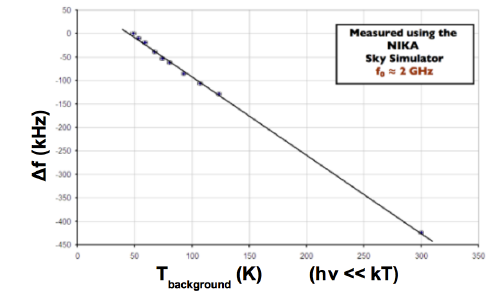
\includegraphics[scale=0.55]{Figures/KID-linearity-Monfardini2014.png}
	\caption{KID linarity demonstrated in laboratory under realistic conditions. Y-axis : frequency shift of the resonance (KID measured signal), X-axis : optical background temperature. The solid line represents the linear fit of the experimental points. Credits : \citet{2014JLTP..176..787M}.}
	\label{KID-lin}
\end{figure}

In the next paragraph we do several simulations following the method described earlier. In these simulations we do a scanning strategy that ensures that the scanning speed is such that the number of points per beam is between 3 and 5 so that we respect Nyquist.

For all simulations we model a planet by simulating a gaussian with amplitudes between 50 and 500 Jy. To see how the non-linearity of the KID progresses we add the CMB dipole and a HWP template. The CMB dipole is a smooth gradient in the CMB temperature accross the sky. It is the result of the motion of the local group of galaxies with respect to the reference framed defined by the CMB. The CMB dipole amplitude is $\Delta T = 3.365 \pm 0.027$ mK and directed toward $(l,b) = (264.4 \degree \pm 0.3 \degree , 48.4 \degree \pm 0.5 \degree)$ in galactic coordinates \citep{2015IJMPD..2430004B}. 

Many experiments, such as MAXIPOL \citep{2007ApJ...665...42J}, EBEX \citep{2010SPIE.7741E..1CR}, POLARBEAR \citep{2017JCAP...05..008T}, \nika2 \citep{2017A&A...599A..34R}, use half-wave plates (HWPs) to improve the sensitivity in polarization measurements by reducing instrumental systematics errors and low-frequency noise. Plus, it allows independant measurements of the three Stokes parameters : I, Q, and U. However, by implementing a HWP, we need to address several issues such as intensity to polarisation leakage and additional parasitic signal peaked at harmonics of the HWP rotation frequency brought by imperfections of the HWP. 

\begin{figure}[h]
\center
	\includegraphics[scale=0.5]{Figures/NL-planet-hwp-dipole.eps}
	\caption{Output flux as a function of Input flux in Jy. 
	The input signal corresponds to a planet, the CMB dipole and a HWP template. Cross and diamond represent the signal reconstructed respectively by \cf and \rf. Black : Output flux as a function of Input flux in Jy. Blue : Scan with 3 points per beam. Red : Scan with 5 points per beam.}
	\label{fig:nl-planet-hwp-dipole}
\end{figure}

Fig \ref{fig:nl-planet-hwp-dipole} shows for the worst case scenario how the non-linearity progresses when we increase the incoming flux from the planet. We can see that the signal is well reconstructed at lower fluxes but becomes non-linear at higher fluxes especially with \rf. Plus, we can see that the more number of points per beam we have the smaller $\varepsilon$ becomes. 

\begin{figure}[h]
\center
	\includegraphics[scale=0.5]{Figures/diff-planet-hwp-dipole-rf.eps}
	\caption{Difference between the output and input signals as a function of the input signal (Jy). Signal were reconstructed with \rf. Diamond, triangle, square and cross correspond respectively to a planet, planet and dipole, planet and HWP template, planet and dipole and HWP template. Blue : Scan with 3 points per beam. Red : Scan with 5 points per beam.}
	\label{fig:diff-rf}
\end{figure}

\begin{figure}[h]
\center
	\includegraphics[scale=0.5]{Figures/diff-planet-hwp-dipole-cf.eps}
	\caption{Difference between the output and input signals as a function of the input signal (Jy). Signal were reconstructed with \cf. Diamond, triangle, square and cross correspond respectively to a planet, planet and dipole, planet and HWP template, planet and dipole and HWP template. Blue : Scan with 3 points per beam. Red : Scan with 5 points per beam.}
	\label{fig:diff-cf}
\end{figure}

The difference between the input signal scanned with 3 and 5 points per beam and the signal reconstructed with \rf and \cf (see Fig \ref{fig:diff-rf} and Fig \ref{fig:diff-cf}) indicates that the signal is better reconstructed when we scan the signal over more points per beam. Plus, it shows that \cf is less limited than \rf at higher flux, as we can see, for \cf the difference stays constant whereas it increases for \rf. 

\begin{table}[h!]
\center
	\begin{tabular}{|c|c|c|}
  	\hline
 	\backslashbox{$\varepsilon$}{$npts/fwhm$} & 3 & 5 \\
	\hline
 	 $\varepsilon_{P}$ & -8.00 x $10^{-5}$ & -7.48 x $10^{-5}$ \\
  	\hline
 	$\varepsilon_{P+D}$ & -8.02 x $10^{-5}$ & -7.50 x $10^{-5}$ \\
  	\hline
  	$\varepsilon_{P+D+HWP}$ & -8.65 x $10^{-5}$ & -8.58 x $10^{-5}$ \\
	\hline
	\end{tabular} 
\caption{Non-linearity coefficients $\varepsilon$ for \rf. The incoming flux corresponds to a planet (500 Jy).}
\label{tab:eps-planet-rf}
\end{table} 

\begin{table}[h!]
\center
	\begin{tabular}{|c|c|c|}
  	\hline
 	\backslashbox{$\varepsilon$}{$npts/fwhm$} & 3 & 5 \\
	\hline
 	$\varepsilon_{P}$ & 6.19 x $10^{-7}$ & 2.82 x $10^{-7}$ \\
  	\hline
 	$\varepsilon_{P+D}$ & 6.16 x $10^{-7}$ & 2.82 x $10^{-7}$ \\
  	\hline
  	$\varepsilon_{P+D+HWP}$ & 4.22 x $10^{-7}$ & 1.70 x $10^{-7}$ \\
	\hline
	\end{tabular} 
\caption{Non-linearity coefficients $\varepsilon$ for \cf. The incoming flux corresponds to a planet (500 Jy).}
\label{tab:eps-planet-cf}
\end{table} 

For all simulation cases we computed the non-linearity coefficient \eps from Eq \ref{eq:fit-nl} (see Tab. \ref{tab:eps-planet-rf} and Tab. \ref{tab:eps-planet-cf}). $\varepsilon$ is smaller when the planet is scanned over more points and when the signal is reconstructed by using \cf. 

To conclude, we can say that both methods \rf and \cf linearly reconstruct the signal even if they become limited at higher flux. Still, the non-linearity coefficients derived by \cf ($\sim 10^{-7}$) are lower than those found with \rf ($\sim 10^{-5}$), meaning that \cf is better than \rf even if it already reconstructed the signal very well.
Plus, we saw that adding a HWP template to an incoming signal consisting of a planet and the CMB dipole only slightly adds non-linearity to the signal and so does not bias the measurement. Moreover, to be able to reconstruct the signal well, we need to put constraints on the scanning speed and so the number of points per beam. In order to do that, we study realistic simulations in the following paragraph, by using a scanning strategy typical of a satellite to scan the Galaxy.
		
\subsubsection{Scanning strategy : Pol sat, PLANCK}
A key factor in the design of space experiments is the scanning strategy of the instrument, as it will play a role in the systematic effects that come from the instrument. Here, we present different simulations of scanning strategies such as the ones used in EPIC \citep{2009arXiv0906.1188B}, and PLANCK \citep{2005A&A...430..363D}. They are represented in Fig \ref{fig:strat-polsat-planck}.

\begin{figure}[h]
\center
	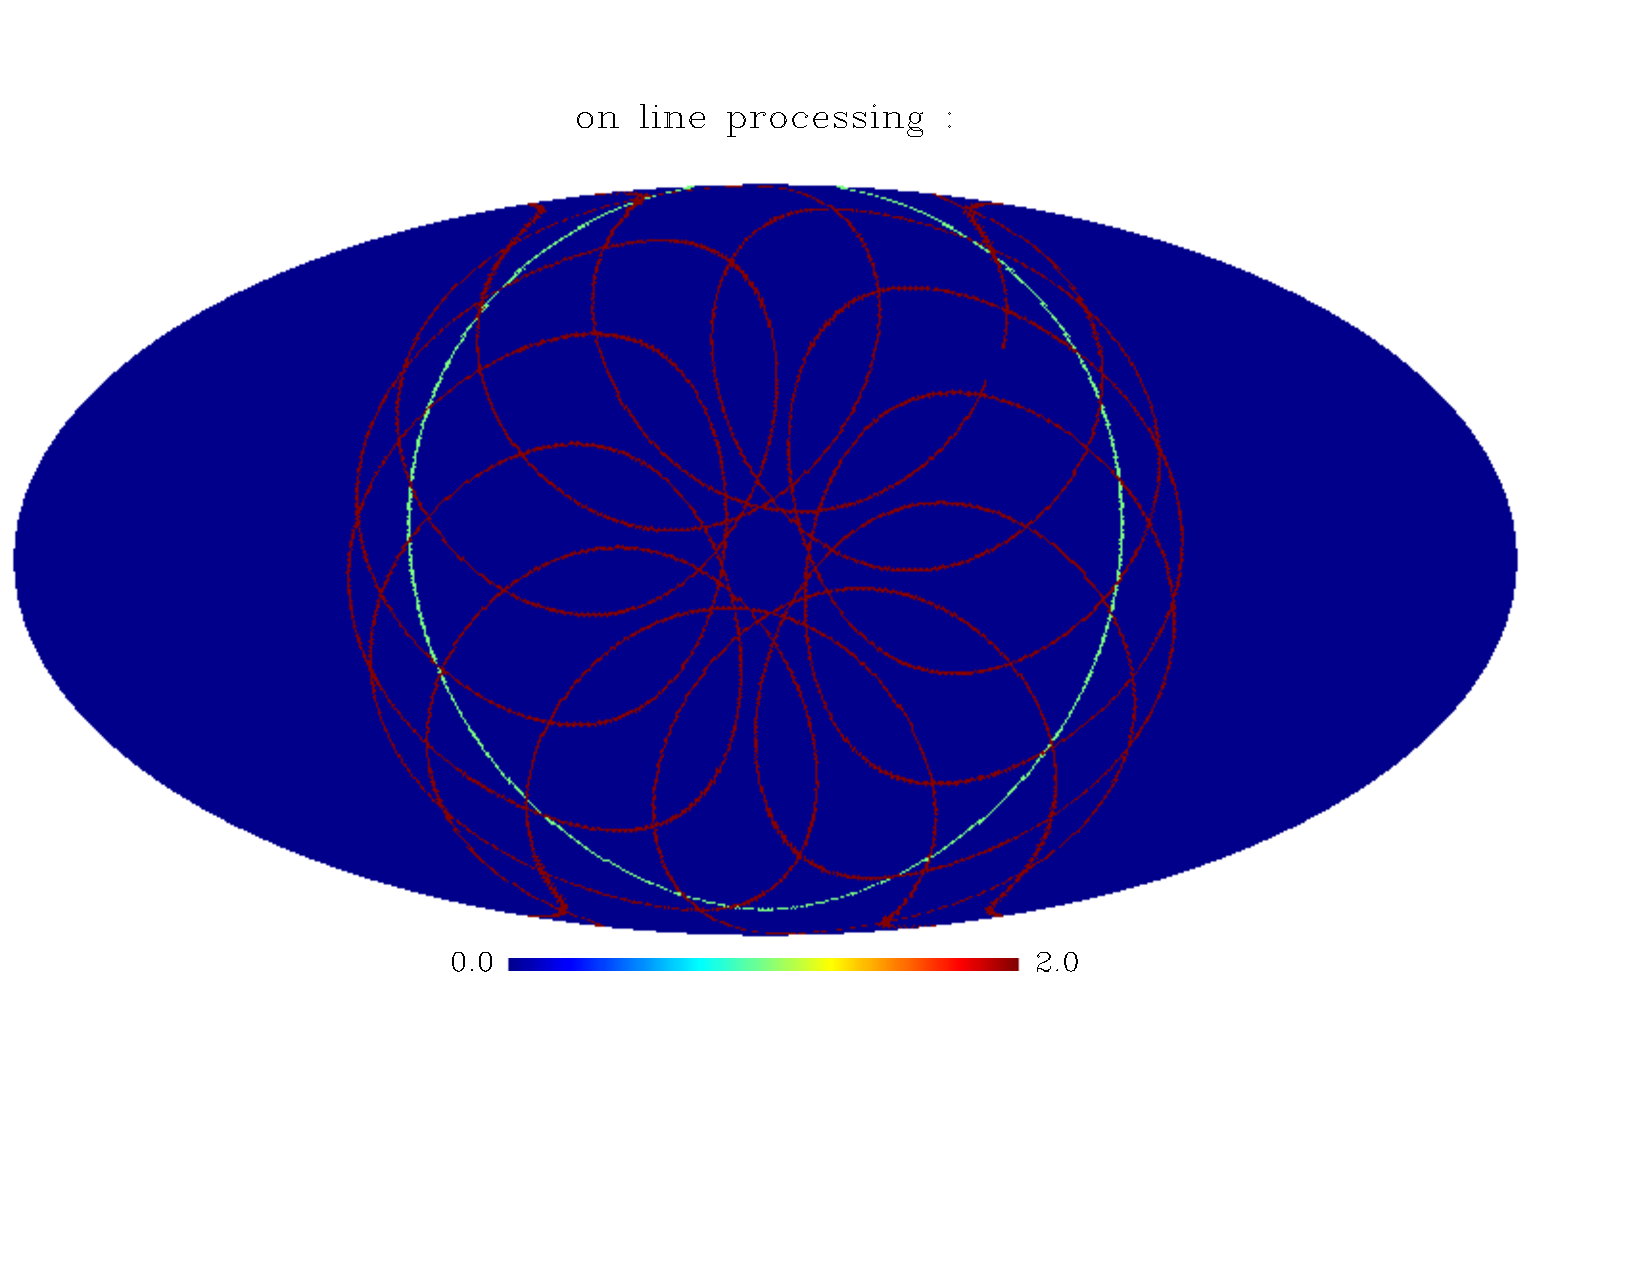
\includegraphics[scale=0.3]{Figures/scan_strat_planck_polsat.pdf}
	\caption{Red : representation of Pol sat scanning strategy. Green : representation of PLANCK scanning strategy }
	\label{fig:strat-polsat-planck}
\end{figure}

For Pol sat scanning strategy, the optical axis of the telescope is inclined by 55 $\degree$ with respect to the spin axis The spin axis is inclined by 45 $\degree$ from the precession axis and it precesses around the Sun-Earth axis every hour.
PLANCK scans large circles on the sky with a 85 $\degree$ angle between the optical axis and the spin axis. The precession angle is 7 $\degree$.

In the next paragraph we will do a more realistic simulation by scanning a map of the Galaxy (REF) and the cosmological dipole, and by using these pointing strategies. We will also add to these maps a HWP template to see if it bias the measurement by inducing non-linearity.

\subsubsection{Results}
In order to derive the non-linearity coefficient in more realistic simulations we scan a map of the Galaxy and the dipole with the two pointing strategies described earlier. Like in the precedent simulations we add the template of a HWP that we subtract after the signal goes through the KID model.

\begin{figure}[h]
\center
	\includegraphics[scale=0.5]{Figures/toi-diff-polsat.eps}
	\caption{Top : Representation of the incoming flux (Galaxy, Dipole and HWP in black), scanned by Pol sat, and its reconstruction using \rf (blue) and \cf (red). Bottom : Difference between the incoming signal and the reconstructed signal.}
	\label{fig:toi-diff-polsat}
\end{figure}

\begin{figure}[h]
\center
	\includegraphics[scale=0.5]{Figures/NL-galaxy-hwp-dipole-polsat.eps}
	\caption{Output flux as a function of Input flux (Galaxy, Dipole and HWP) in Jy. We used Pol sat scanning strategy. Red : The signal was reconstructed with \cf. Blue : The signal was reconstructed with \rf.}
	\label{fig:nl-galaxy-hwp-dipole-polsat}
\end{figure}

In Fig. \ref{fig:toi-diff-polsat} we reconstructed the signal of the Galaxy, dipole and hwp and we can see in Fig. \ref{fig:nl-galaxy-hwp-dipole-polsat} that it was linearly reconstructed. 
In the next part we did the same simulations but we used Planck scanning strategy. The results are shown Fig. \ref{fig:toi-diff-planck} and Fig. \ref{fig:nl-galaxy-hwp-dipole-planck}. PROBLEME

\begin{figure}[h]
\center
	\includegraphics[scale=0.5]{Figures/toi-diff-planck.eps}
	\caption{Top : Representation of the incoming flux (Galaxy, Dipole and HWP in black), scanned by PLANCK, and its reconstruction using \rf (blue) and \cf (red). Bottom : Difference between the incoming signal and the reconstructed signal. }
	\label{fig:toi-diff-planck}
\end{figure}

\begin{figure}[h]
\center
	\includegraphics[scale=0.5]{Figures/NL-galaxy-hwp-dipole-planck.eps}
	\caption{Output flux as a function of Input flux (Galaxy, Dipole and HWP) in Jy.We used PLANCK scanning strategy. Red : The signal was reconstructed with \cf. Blue : The signal was reconstructed with \rf.}
	\label{fig:nl-galaxy-hwp-dipole-planck}
\end{figure}

\begin{table}[h!]
\center
	\begin{tabular}{|c|c|c|}
  	\hline
 	\backslashbox{$\varepsilon$}{$Input signal$} & $	\varepsilon_{R_{f}}$ & $\varepsilon_{C_{f}} $ \\
	\hline
	$G$  & 1.88 x $10^{-7}$ & -2.03 x $10^{-8}$ \\
 	\hline
 	$G+D$  & 2.35 x $10^{-4}$ & 2.35 x $10^{-4}$ \\
  	\hline
 	$G+D+HWP$ & 1.24 x $10^{-3}$ & 2.34 x $10^{-4}$ \\
  	\hline
	\end{tabular} 
\caption{Non-linearity coefficients \eps for \rf and \cf derived for Pol sat scanning strategy. $G$, $D$ and $HWP$ respectively stands for Galaxy, Dipole and Half Wave Plate.}
\label{tab:eps-galaxy-hwp-dipole-polsat}
\end{table}

In Tab. \ref{tab:eps-galaxy-hwp-dipole-polsat} we can see that for both pointing strategies the non-linearity coefficients are higher when we add the dipole and HWP to the input signal. In addition, they emphasize the fact that the \cf method of signal reconstruction is slightly better than \rf, which confirms what we saw with the planet simulation.\\

To conclude, KIDs are a promising new type of technology. Here, we studied the KID response to several sources such as a planet, the CMB dipole and a signal from a HWP. We observed that we needed to put constraints on the scanning strategy, consequently we did more realistic simulations by scanning a map of the Galaxy and the dipole, by using the scanning strategy of a satellite (Pol Sat, PLANCK). In all the simulations, we have seen that the response of a KID is linear. In fact, the non-linearity coefficients that we derived are low (\eps $\simeq 10^{-3} - 10^{-7}$). But this linearity depends on the scanning strategy and on the method used to reconstruct the signal. Indeed, even if both methods, \rf and \cf, can reconstruct the signal very well, \cf is less limited than \rf when the KID is submitted to high fluxes.
In this section we have seen that KIDs are capable of reproducing with fidelity the incoming signal in the context of a space mission. In the next section, we will apply this to the study of the CMB. 

\section{Application to CMB maps and power spectra estimations}
The measurement of CMB polarization, and especially the detection of $B$ modes, is one of the major challenges in modern cosmology. In this section, we show that the KIDs systematic effect such as the non-linearity does not affect them from detecting $B$ modes.\\

A measure done by a KID is defined by $m = T + P$, with $T$ and $P$ representing the temperature and polarization. We will focus on the non-linear terms produced by the detector which is characterized by the $\varepsilon$ coefficient in $ m = m_{1} + \varepsilon m_{1}^{2}$. We have : 

\begin{equation}
\begin{split}
m & = m_{1} +\varepsilon' (T+P)^{2} \\
 & = T + P + \varepsilon'(T^{2} + P^{2} + 2TP) 
\end{split}
\end{equation}

Therefore, knowing that $T=I$ and $P = Q\cos(2\alpha) + U \sin(2\alpha)$, the polarized equation with a non-linear term is given Eq. \ref{eq:eq-NL}.

\begin{equation}
m  \simeq (I + \varepsilon' I^{2}) + (Q + 2\varepsilon' IQ) \cos(2\alpha) + (U + 2 \varepsilon' IU) \sin(2\alpha)
\label{eq:eq-NL}
\end{equation}

The non-linearity coefficient depends on the detector response. In fact, it is a systematic effect of the instrument and as a consequence will always impact our measurements. This non-linearity can lead to leakage of the CMB and dust temperature signal into the polarization maps and consequently can induce spurious polarization signals which could prevent us from detecting $B$ mode polarization. 
To study this effect we simulate spurious signals from a map of the galaxy (dust) observed by PLANCK (REF) by applying the non-linear mapping described by Eq. \ref{eq:spurious-mapI}, \ref{eq:spurious-mapQ}, \ref{eq:spurious-mapU} from Eq. \ref{eq:eq-NL}.

\begin{eqnarray}
\label{eq:spurious-mapI}
\Delta I_{dust}  &=& \varepsilon I_{dust}^{2},\\
\label{eq:spurious-mapQ}
\Delta Q_{dust}  &=& 2\varepsilon I_{dust}Q_{dust},\\
\label{eq:spurious-mapU}
\Delta U_{dust} &=& 2 \varepsilon I_{dust}U_{dust},
\end{eqnarray}

Then, to investigate the different modes of CMB polarization we used the HEALPix package \citep{2005ApJ...622..759G} to generate modified power spectra from the spurious polarization maps. They are described by Eq. \ref{eq:eq-cl} and are represented in Fig. \ref{fig:cl2}.

\begin{equation}
\Delta C_{l} = \varepsilon'^{2} C_{l}^{XX'},
\label{eq:eq-cl}
\end{equation}
Where $\lbrace X,X' \rbrace$ = $\lbrace T,E,B \rbrace$ .\\

\begin{figure}[h]
\center
	\includegraphics[scale=0.55]{Figures/cl2.eps}
	\caption{Power spectra for spurious temperature and polarization anisotropies. The black, blue, red and green curves indicate the $TT$, $TE$, $EE$ and $BB$ power spectra. The bottom three green curves represents the $BB$ power spectra for a tensor-to-scalar ratio r = (T/S) = 0.1, 0.01, 0.001.}
	\label{fig:cl2}
\end{figure}

Here we will focus on : 
\begin{equation}
\Delta C_{l} = \varepsilon'^{2} C_{l}^{TE}.
\label{eq:eq-cl2}
\end{equation}

The leakage of temperature into polarization is represented by the coefficient $\varepsilon'$ of Eq. \ref{eq:eq-cl2}. To determine this coefficient, we compute :

\begin{equation}
\varepsilon' = \sqrt{\dfrac{r}{C_{l}^{TE}}},
\label{eq:eq-cl3}
\end{equation}

they are represented in Tab. \ref{tab:eps-lkg}

\begin{table}[h!]
\center
	\begin{tabular}{|c|c|c|c|}
  	\hline
 	\backslashbox{$\varepsilon'$}{$r$} & 0.1 & 0.01 & 0.001 \\
	\hline
	$\varepsilon'$ & 2.51 x $10^{-2}$ & 7.95 x $10^{-3}$ & 2.51 x $10^{-3}$\\
  	\hline
	\end{tabular} 
\caption{Non-linear coefficients related to the leakage of temperature into polarization for scalar-to-tensor ratio r = (T/S) = 0.1, 0.01, 0.001.}
\label{tab:eps-lkg}
\end{table}

To be able to detect $B$ mode polarization without being contaminated by the leakage of temperature into polarization, the non-linearity coefficient related to the detector and the signal reconstruction must be lower than $\varepsilon'$. 
By comparing Tab. \ref{tab:eps-galaxy-hwp-dipole-polsat} and Tab. \ref{tab:eps-lkg} we can see that the non-linearity coefficients related to the instrument are lower than the coefficients related to the leakage, consequently considering the KID systematic effect it is possible to detect the CMB polarization without being contaminated by the leakage of temperature into polarization.\\

To conclude, the sudy of CMB polarization and the measurement of $B$ modes polarization represent one of the major challenges in modern cosmology. The detection of $B$ modes can be affected by a leakage effect of temperature into polarization. Here we studied the non-linearities that the leakage from dust temperature can create. We have seen that the non-linearity coefficients linked to the detector response are ranged between $10^{-3}$ and $10^{-8}$, which are lower than the non-linearity coefficients related to the leakage ($\simeq 10^{-2} - 10^{-3}$). So the KID is capable of detecting the signal of B mode polarization that is not contaminated by the leakage effect.

\section{Cosmic rays impact on KIDs array}

One of the major problems for space based missions is the impact of an intense flux of high energy particles, referred to as Cosmic Rays (CR) on the detectors. Primary CR are produced by the Sun and by other galactic sources. They are mostly composed by protons (90\%), helium nuclei (9\%) and a few heavier nuclei and electrons (1\%). The CR spectrum is peaked aroud 200 MeV, thus the particles have sufficient energy to penetrate the detectors and give an unwanted signal. The Planck satellite \citep{2014A&A...571A..10P} has demonstrated that the impact of CR on the detectors are a key problem for space missions. Indeed, the glitches caused by CR can mask the real data and induce a loss of an important fraction of it.\\
Experiments have been done to construct a setup that allows to study the behavior of KIDs arrays under typical conditions of a space-borne observatory, and establish the compatibility of KIDs with a space environment \citep{2016A&A...592A..26C,2016SPIE.9914E..0NM}. When the detector is hit by a CR there is a lapse of time during which the sensor is 'blind' to the incoming scientific data. The length of this dead-time depends on the response time of the KID (time constant) which is determined by the quasi particle lifetime. \citet{2012ApPhL.100w2601M} have shown for KID, this time constant is equal to about tens of microseconds which is faster than bolometers (from 5-10 ms to 2s). This means that for the same CR hit, less data is lost when using KIDs arrays. Plus, the experiments have confirmed the fact that KID recover their initial state in less than 5 milliseconds. Finally, \citet{2016SPIE.9914E..0NM} concluded that the percent level of data loss per pixel by a KIDs array placed in a space environment is about 1 \% compared to 15 \% for Planck HFI bolometers.\\ The KID technology shows promising results for compatibility with a space-borne mission, as their extremely short glitch time constant permits to greatly reduce the data loss fraction due to CR impacts. 

